\documentclass{beamer}
\usepackage[utf8]{inputenc}
\usepackage[english]{babel}
\usepackage[T1]{fontenc}
\usepackage{multimedia}
\usepackage[absolute,overlay]{textpos}
\usepackage{graphicx}
\usepackage{tikz}
\usepackage{times}
\usepackage{amsmath}
\usepackage{verbatim}
\usepackage{xcolor}
\usepackage{textpos}
\usepackage{eulervm}

\let\oldmb\mathbold
\protected\def\mathbold{\oldmb}
\usetikzlibrary{arrows,shapes}
\usetikzlibrary{patterns,arrows,decorations.pathreplacing}
\usetheme{Darmstadt}
\usecolortheme{lily}

\pagenumbering{arabic}\setcounter{page}{1}

\author[The author]{Fabrizio Grosa}
\institute[Inst.]{University of Turin, Italy \\\vspace{0.5cm} GSI Summer Student Program 2014}%{\includegraphics[scale=0.35]{uni.pdf}\\University of Turin, Italia}
\title{Heavy-flavour production}
\subtitle{Estimation of $\gamma$, \space $\pi^{0}$ and $\eta$ ratios in the photonic background in proton-proton collisions at $\sqrt{s} = 
7$ TeV with ALICE}

\logo{
  \includegraphics[width=1.5cm,height=1.5cm,keepaspectratio]{logo.jpg}
   }
   
\date{\vspace{-5ex}}

\begin{document}

\begin{frame}
\maketitle
\end{frame}

\begin{frame}
\frametitle{Outline}
\tableofcontents
\end{frame}

\section{Heavy-flavour production in heavy-ion collisions}
\begin{frame}
\frametitle{Quark-gluon plasma}
\begin{picture}(320,250)

\put(0,145){\includegraphics[scale=0.35]{evolution.jpg}}

\put(-10,250){
\begin{minipage}[t]{1\linewidth}
\footnotesize
\begin{itemize}
\item QCD predicts that under extreme conditions of very high temperature or energy densities, hadronic matter 
transit to a deconfined phase of matter called \textit{``quark-gluon plasma``} (QGP)
\end{itemize}
\end{minipage}}

\put(300,210){
\begin{minipage}[t]{0.5\linewidth}
\textbf{t}
\end{minipage}}

\put(0,205){
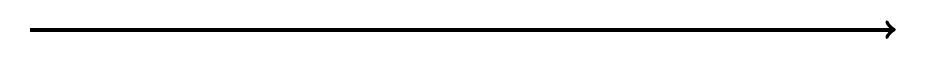
\begin{tikzpicture}[->]
\draw[draw=black,solid,line width=0.5mm] (1, 1) -- + (11, 0);
\end{tikzpicture}}

\put(-20,130){
\begin{minipage}[t]{0.5\linewidth}
\begin{itemize}
\footnotesize
\item \textbf{Collision}: large number of hard scatterings between partons.
\item \textbf{Thermalization} : the thermal equilibrium is reached.
\item \textbf{QGP}: the fireball is created, in which quarks and gluons are free.
\end{itemize}
\end{minipage}}

\put(150,130){
\begin{minipage}[t]{0.5\linewidth}
\begin{itemize}
\footnotesize
\item \textbf{Hadronization} : the quarks and the glouns are recombined in hadrons.
\item \textbf{Chemical freeze-out}: inelastic scattering cease.
\item \textbf{Kinetic freeze-out} : elastic scattering cease.
\end{itemize}
\end{minipage}}

\end{picture}
\end{frame}

\begin{frame}
 \frametitle{Heavy-flavour production}
\begin{picture}(320,250)

\put(-10,130){\includegraphics[scale=0.11]{cone_and_hf.png}}

\put(120,240){
\begin{minipage}[t]{0.6\linewidth}
\begin{itemize}
\footnotesize
\item Heavy-flavour production happens through initial hard partonic scattering processes when the medium is more dense
\item Heavy-flavour quarks lose energy travelling in the QGP 
\end{itemize}
\end{minipage}}

\put(25,50){\includegraphics[scale=0.3]{semileptonic.jpg}}

\put(235,145){

\begin{tikzpicture}[->]
\draw[draw=blue,solid,line width=0.7mm] (1, 1) -- + (1., -1);
\end{tikzpicture}}

\put(250,130){
\begin{minipage}[t]{0.3\linewidth}
\footnotesize
Probe for the QGP
\end{minipage}}

\put(10,110){
\begin{minipage}[t]{0.5\linewidth}
\textcolor{blue}{\it semileptonic decay}
\end{minipage}}

\end{picture}
\end{frame}

\begin{frame}
\frametitle{Background of heavy-flavour hadron decays} 
\begin{picture}(320,250)

\put(0,40){\includegraphics[scale=0.08]{2013-Jan-03-inclusive_versus_cocktail_combined_mult.png}}

\put(145,160){
\begin{minipage}{0.55\linewidth}
\footnotesize
\begin{itemize}
 \item There are other sources of leptons which form the background for the heavy-flavour hadron semileptonic decay. 
 \item The \textit{inclusive} electrons and positrons are all the $e^{\pm}$ measured, which are decay products of both 
 hadrons carrying heavy quarks, and the background sources.
 \item After the subtraction of the background only the remaining $p_{T}$ spectrum contains electrons from heavy-flavour hadron
 decays only.
\end{itemize}
\end{minipage}}

\end{picture}
\end{frame}

\section{Photonic background}
\begin{frame}
\frametitle{Main sources of the photonic background} 
\begin{picture}(320,250)

\put(-10,70){\includegraphics[scale=0.5]{dalitz.jpg}}
\put(-10,170){\includegraphics[scale=0.2]{conversion.jpg}}

\put(130,173){
\begin{minipage}{0.8\linewidth}
\begin{itemize}
\item 
Photon conversion: $\gamma \rightarrow e^{+}e^{-}$ 
\vspace{1.5cm}
\item
Dalitz decays: 
\end{itemize}
\end{minipage}}

\put(230,115){
\begin{minipage}{0.4\linewidth}
{$\pi^{0} \rightarrow e^{+}e^{-}\gamma$\\$\eta \rightarrow e^{+}e^{-}\gamma$\\
$\eta' \rightarrow e^{+}e^{-}\gamma$\\$\omega \rightarrow e^{+}e^{-}\pi_{0}$\\$\phi \rightarrow e^{+}e^{-}\eta$}
\end{minipage}}

\pause
\put(225,123){

\begin{tikzpicture}[-]
\draw[draw=blue,solid,line width=0.2mm] (0,0) -- (2.5,0) -- (2.5,1.05) -- (0,1.05) -- (0,0);
\end{tikzpicture}}

\put(247,198){

\begin{tikzpicture}[-]
\draw[draw=blue,solid,line width=0.2mm] (0,0) -- (1.9,0) -- (1.9,0.5) -- (0,0.5) -- (0,0);
\end{tikzpicture}}

\put(0,60){
%\footnotesize
\begin{minipage}{1\linewidth}
\textcolor{blue}{The aim of this study is to calculate the ratio between photon conversions and Dalitz decays in the 
photonic background}
\end{minipage}}

\end{picture}
\end{frame}

\begin{frame}
 \frametitle{The ALICE detector}
\begin{picture}(320,250)

\put(-10,50){\includegraphics[scale=0.45]{ALICE_detector.jpg}}
\put(210,140){\includegraphics[scale=0.16]{ITS_TPC.jpg}}

\put(0,210){
\begin{minipage}{0.7\linewidth}
\begin{itemize}
\item ALICE is the experiment at LHC dedicated to heavy-ion collisions 
\end{itemize}
\end{minipage}}

\put(160,100){
\begin{minipage}{0.55\linewidth}
\footnotesize
\begin{itemize}
\item \textbf{I}nner \textbf{T}racking \textbf{S}ystem: \\first sub detector reached by the particles originating in the primary vertex 
\item \textbf{T}ime \textbf{P}rojection \textbf{C}hamber: \\the main tracking detector 
\end{itemize}
\end{minipage}}

\end{picture}
\end{frame}

\begin{frame}
\frametitle{Data samples}
\begin{picture}(320,250)

\put(0,150){
\begin{minipage}{1\linewidth}
\begin{itemize}
\setlength{\itemsep}{7pt}
\item simulated proton-proton collision events at $\sqrt{s} = 7 TeV$
\vspace{0.3cm}
 \begin{itemize}
   \setlength{\itemsep}{7pt}
 \item decayed with \textit{Pythia 6}
 \item propagation through detectors described with \textit{\textbf{GE}ometry \textbf{AN}d \textbf{T}racking} 3
 \item tracks reconstructed with AliROOT
\end{itemize}
\item this study is focused on proton-proton collisions because they are the reference system for the Pb-Pb collisions
\end{itemize}
\end{minipage}}

\end{picture}
\end{frame}

\begin{frame}
\frametitle{$e^{\pm}$ identification}
\begin{picture}(320,250)

\put(-10,35){\includegraphics[scale=0.45]{incl-ass.pdf}}

\put(-30,230){
\begin{minipage}{0.6\linewidth}
\begin{itemize}
\footnotesize
 \item Inclusive $e^{\pm}$
\end{itemize}
\end{minipage}}

\put(130,230){
\begin{minipage}{0.6\linewidth}
\begin{itemize}
\footnotesize
 \item Associated $e^{\pm}$
\end{itemize}
\end{minipage}}

\put(42,230){
\begin{tikzpicture}[->]
\draw[draw=blue,solid,line width=0.5mm] (1, 1) -- + (0.5, 0);
\draw[draw=blue,solid,line width=0.5mm] (7., 1) -- + (0.5, 0);
\end{tikzpicture}}

\put(62,223){
\begin{minipage}{0.3\linewidth}
\footnotesize
{stringent cuts are \\required} 
\end{minipage}}

\put(235,207){
\begin{minipage}{0.3\linewidth}
\footnotesize
{relaxed cuts are \\required:\\tracks resolution is lost,\\ but efficiency is maximised} 
\end{minipage}}

\put(230,115){
\begin{minipage}{0.3\linewidth}
\footnotesize
Finally, using the MC truth information, only the tracks that really belong to $e^{\pm}$ are selected
\end{minipage}}

\end{picture}
\end{frame}

\begin{frame}
\frametitle{Invariant mass analysis}
\begin{picture}(320,250)

\put(0,220){
\begin{minipage}{1\linewidth}
{According to Special Relativity the four-momentum \\$p = (E, \vec{p})$ of a physics system is always conserved, and 
the mass of a particle is equal to:}
\end{minipage}}

\put(30,175){
\begin{minipage}{1\linewidth}
{\fcolorbox{blue}{white}{$m_{i}^{2} = E_{i}^{2}-\vec{p_{i}}^{2} 
\equiv p_{i}^{2}$}}
\end{minipage}}

\put(0,138){
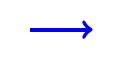
\begin{tikzpicture}[->]
\draw[draw=blue,solid,line width=0.5mm] (1, 1) -- + (0.8, 0);
\end{tikzpicture}}

\put(30,135){
\begin{minipage}{0.8\linewidth}
{we can calculate the invariant mass of a particle from its decay products}
\end{minipage}}

\put(50,100){
\begin{minipage}{1\linewidth}
{\fcolorbox{blue}{white}{
$m_{ee} = \sqrt{(p_{1}+p_{2})^{2}} = \sqrt{(E_{1}+E_{2})^{2}-(\vec{p_{1}}+\vec{p_{2}})^{2}}$}} 
\end{minipage}}

\end{picture}
\end{frame}

\begin{frame}
\frametitle{Invariant mass distributions from MC truth} 
\begin{picture}(320,250)

\put(-20,237){
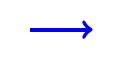
\begin{tikzpicture}[->]
\draw[draw=blue,solid,line width=0.5mm] (1, 1) -- + (0.8, 0);
\end{tikzpicture}}

\put(55,232){
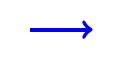
\begin{tikzpicture}[->]
\draw[draw=blue,solid,line width=0.5mm] (1, 1) -- + (0.8, 0);
\end{tikzpicture}}

\put(10,235){
\footnotesize
\begin{minipage}{1\linewidth}
Using the MC truth information is possible to know the mother particle of every $e^{+}e^{-}$ pair
\end{minipage}}

\put(85,230){
\footnotesize
\begin{minipage}{0.7\linewidth}
obtained the invariant mass distribution of each source
\end{minipage}}

\put(-20,50){\includegraphics[scale=0.5]{sources.pdf}}

\put(20,207){
\footnotesize
\begin{minipage}{1\linewidth}
\textcolor{green}{\Large{$\gamma$}}
\end{minipage}}

\put(115,207){
\footnotesize
\begin{minipage}{1\linewidth}
\textcolor{black}{\Large{$\pi^{0}$}}
\end{minipage}}

\put(210,207){
\footnotesize
\begin{minipage}{1\linewidth}
\textcolor{blue}{\Large{$\eta$}}
\end{minipage}}

\put(260,170){
\begin{minipage}{0.3\linewidth}
\textcolor{blue}{MC truth}
\end{minipage}}

\put(260,90){
\begin{minipage}{0.3\linewidth}
\textcolor{blue}{MC \\reconstructed}
\end{minipage}}

\end{picture}
\end{frame}

\begin{frame}
\frametitle{Distribution for photons} 
\begin{picture}(320,250)

\put(50,40){\includegraphics[scale=0.38]{gamma_temp.pdf}}

\put(111,231){
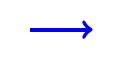
\begin{tikzpicture}[->]
\draw[draw=blue,solid,line width=0.5mm] (1, 1) -- + (0.8, 0);
\end{tikzpicture}}

\put(-20,230){
\footnotesize
\begin{minipage}{1.5\linewidth}
\begin{itemize}
 \item For the photon conversion \hspace{1 cm} exponentially modified Gaussian distribution:
\end{itemize}
\end{minipage}}

\put(-63,200){
\begin{minipage}{1\linewidth}
\footnotesize
\begin{equation*}
\frac{dN}{dm_{ee}}=N_{\gamma}\cdot e^{-\frac{(m_{ee}-M_{\gamma})^{2}}{2\sigma^{2}}}+\Theta(m_{ee}-M_{\gamma})
e^{\frac{m_{ee}-M_{\gamma}}{\tau}}
\end{equation*}
\end{minipage}}

\end{picture}
\end{frame}

\begin{frame}
\frametitle{Kroll-Wada distribution}
\begin{picture}(320,250)

\put(-10,40){\includegraphics[scale=0.38]{dalitz_temp.pdf}}

\put(91,231){
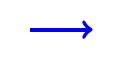
\begin{tikzpicture}[->]
\draw[draw=blue,solid,line width=0.5mm] (1, 1) -- + (0.8, 0);
\end{tikzpicture}}

\put(-20,230){
\footnotesize
\begin{minipage}{1\linewidth}
\begin{itemize}
 \item For the Dalitz decays \hspace{1 cm} Kroll-Wada distribution:
\end{itemize}
\end{minipage}}

\put(-10,210){
\begin{minipage}{1\linewidth}
\fontsize{7}{2}
\begin{equation*}
 \frac{dN}{dm_{ee}} = N_{X}\cdot\frac{2}{m_{ee}}\Bigg\{(1+(m_{ee}/M_{X})^{2})^2-4(m_{ee}/M_{X})^{2}
\Bigg\}^{3/2}\sqrt{1-\frac{4(m_{e}/M_{X})^{2}}{(m_{ee}/M_{X})^{2}}}\cdot
 \Bigg\{1+\frac{2(m_{e}/M_{X})^{2}}{(m_{ee}/M_{X})^{2}}\Bigg\}\cdot F_{X}(m_{ee}^2)
\end{equation*}
\end{minipage}}

\put(120,140){
\begin{minipage}{1\linewidth}
\footnotesize
\begin{equation*}
\Bigg \{
\begin{array}{rl}
F_{\pi^{0}}(m_{ee}^2) = \frac{1}{(1-5.5\cdot m_{ee}^2)^{2}}\\
F_{\eta}(m_{ee}^2) = \frac{1}{(1-1.9\cdot m_{ee}^2)^{2}}
\end{array}
\end{equation*}
\end{minipage}}

\put(190,140){
\footnotesize
\begin{minipage}{1\linewidth}
where
\end{minipage}}

\end{picture}
\end{frame}


\begin{frame}
\frametitle{Fit template} 
\begin{picture}(320,250)

\put(-30,220){
\footnotesize
\begin{minipage}{1\linewidth}
\begin{itemize}
 \item Select $e^{+}e^{-}$ pair with same $\gamma$, \space $\pi^{0}$ or $\eta$ mother particle from MC truth 
 \item Calculate their invariant mass and obtain the relative distribution
 \item Fit with the function which is the sum of the three contributions
 \end{itemize}
\end{minipage}}

\put(-20,40){\includegraphics[scale=0.38]{Inv_mass_ESD.pdf}}

\put(235,190){
\footnotesize
\begin{minipage}{1\linewidth}
\textcolor{blue}{From MC truth}
\end{minipage}}

\put(110,162){
\begin{minipage}{1\linewidth}
\begin{table}[htpb]
\center
\fontsize{10}{3}
\scalebox{0.48}{
\begin{tabular}{|c|c|c|}
  \hline
  \raisebox{0pt}[10pt][4pt]{number of $\gamma$} &
  \raisebox{0pt}[10pt][4pt]{418300 $\pm$ 600} \\
  \hline
  \raisebox{0pt}[10pt][4pt]{number of $\pi^{0}$} &
  \raisebox{0pt}[10pt][4pt]{362000 $\pm$ 600} \\
  \hline
  \raisebox{0pt}[10pt][4pt]{number of $\eta$} &
  \raisebox{0pt}[10pt][4pt]{42100 $\pm$ 200} \\
  \hline
  \raisebox{0pt}[10pt][4pt]{$n_{\gamma}/ n_{\pi^{0}}$} &
  \raisebox{0pt}[10pt][4pt]{1.156 $\pm$ 0.003} \\
  \hline
  \raisebox{0pt}[10pt][4pt]{$n_{\gamma}/ n_{\eta}$} &
  \raisebox{0pt}[10pt][4pt]{9.94 $\pm$ 0.05} \\
  \hline
  \raisebox{0pt}[10pt][4pt]{$n_{\gamma}/(n_{\pi^{0}}+n_{\eta})$} &
  \raisebox{0pt}[10pt][4pt]{1.035 $\pm$ 0.002} \\
  \hline
  \end{tabular}}
\end{table}
\end{minipage}}

\put(230,128){
\footnotesize
\begin{minipage}{1\linewidth}
\textcolor{blue}{From the Fit}
\end{minipage}}

\put(100,90){
\begin{minipage}{1\linewidth}
\begin{table}[htpb]
\center
\fontsize{10}{3}
\scalebox{0.48}{
\begin{tabular}{|c|c|c|}
   \hline
  \raisebox{0pt}[10pt][4pt]{$M_{\gamma}$} &
  \raisebox{0pt}[10pt][4pt]{0.01107 $\pm$ 0.00018 $GeV/c^{2}$} \\
  \hline
  \raisebox{0pt}[10pt][4pt]{$M_{\pi^{0}}$} &
  \raisebox{0pt}[10pt][4pt]{0.1611 $\pm$ 0.0003 $GeV/c^{2}$} \\
  \hline
  \raisebox{0pt}[10pt][4pt]{$M_{\eta}$} &
  \raisebox{0pt}[10pt][4pt]{0.558 $\pm$ 0.004 $GeV/c^{2}$} \\
  \hline
  \raisebox{0pt}[10pt][4pt]{Integral of $\gamma$ } &
  \raisebox{0pt}[10pt][4pt]{418300 $\pm$ 1100} \\
  \hline
  \raisebox{0pt}[10pt][4pt]{Integral of $\pi^{0}$ } &
  \raisebox{0pt}[10pt][4pt]{355000 $\pm$ 2000} \\
  \hline
  \raisebox{0pt}[10pt][4pt]{Integral of $\eta$ } &
  \raisebox{0pt}[10pt][4pt]{49200 $\pm$ 600} \\
  \hline
  \raisebox{0pt}[10pt][4pt]{$I_{\gamma}/I_{\pi^{0}}$} &
  \raisebox{0pt}[10pt][4pt]{1.179 $\pm$ 0.007} \\
  \hline
  \raisebox{0pt}[10pt][4pt]{$I_{\gamma}/I_{\eta}$} &
  \raisebox{0pt}[10pt][4pt]{8.50 $\pm$ 0.11} \\
  \hline
  \raisebox{0pt}[10pt][4pt]{$I_{\gamma}/(I_{\pi^{0}}+I_{\eta})$} &
  \raisebox{0pt}[10pt][4pt]{1.035 $\pm$ 0.006} \\
  \hline
  \end{tabular}}
\end{table}
\end{minipage}}

\end{picture}
\end{frame}

\begin{frame}
\frametitle{Like-sign and Unlike-sign distributions} 
\begin{picture}(320,250)

\put(50,40){\includegraphics[scale=0.37]{like-unlike_norm.pdf}}

\put(-30,230){
\begin{minipage}{1\linewidth}
\begin{itemize}
 \item Unlike-sign distribution  
 \end{itemize}
\end{minipage}}

\put(150,230){
\begin{minipage}{1\linewidth}
\begin{itemize}
 \item Like-sign distribution  
 \end{itemize}
\end{minipage}}

\put(-15,215){
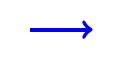
\begin{tikzpicture}[->]
\draw[draw=blue,solid,line width=0.5mm] (1, 1) -- + (0.8, 0);
\end{tikzpicture}}

\put(165,215){
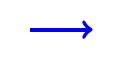
\begin{tikzpicture}[->]
\draw[draw=blue,solid,line width=0.5mm] (1, 1) -- + (0.8, 0);
\end{tikzpicture}}

\put(15,215){
\begin{minipage}{1\linewidth}
\footnotesize
inclusive $e^{\pm}$ + associated $e^{\mp}$
\end{minipage}}

\put(195,215){
\begin{minipage}{1\linewidth}
\footnotesize
inclusive $e^{\pm}$ + associated $e^{\pm}$
\end{minipage}}

\put(-5,200){
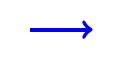
\begin{tikzpicture}[->]
\draw[draw=blue,solid,line width=0.5mm] (1, 1) -- + (0.8, 0);
\end{tikzpicture}}

\put(175,200){
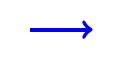
\begin{tikzpicture}[->]
\draw[draw=blue,solid,line width=0.5mm] (1, 1) -- + (0.8, 0);
\end{tikzpicture}}

\put(25,192){
\begin{minipage}{1\linewidth}
\footnotesize
photonic signal + \\combinatorial background
\end{minipage}}

\put(205,198){
\begin{minipage}{1\linewidth}
\footnotesize
combinatorial background
\end{minipage}}

\end{picture}
\end{frame}

\begin{frame}
\frametitle{Fit of the photonic background} 
\begin{picture}(320,250)

\put(-30,230){
\begin{minipage}{1.2\linewidth}
\begin{itemize}
 \item The like-sign distribution is subtracted to the unlike-sign distribution 
 \end{itemize}
\end{minipage}}

\put(-20,50){\includegraphics[scale=0.42]{esd_comb.pdf}}

\put(200,180){
\begin{minipage}{0.4\linewidth}
\footnotesize
\begin{itemize}
 \item The resulting photonic signal is fitted with the template obtained from the MC truth
 \end{itemize}
\end{minipage}}

\put(110,110){
\begin{minipage}{1\linewidth}
\begin{table}[htpb]
\center
\fontsize{10}{3}
\scalebox{0.6}{
\begin{tabular}{|c|c|c|}
  \hline
  \raisebox{0pt}[10pt][4pt]{Integral of $\gamma$ } &
  \raisebox{0pt}[10pt][4pt]{423000 $\pm$ 6000} \\
  \hline
  \raisebox{0pt}[10pt][4pt]{Integral of $\pi^{0}$ } &
  \raisebox{0pt}[10pt][4pt]{354000 $\pm$ 4000} \\
  \hline
  \raisebox{0pt}[10pt][4pt]{Integral of $\eta$ } &
  \raisebox{0pt}[10pt][4pt]{42000 $\pm$ 3000} \\
  \hline
  \raisebox{0pt}[10pt][4pt]{$I_{\gamma}/I_{\pi^{0}}$} &
  \raisebox{0pt}[10pt][4pt]{1.19 $\pm$ 0.02} \\
  \hline
  \raisebox{0pt}[10pt][4pt]{$I_{\gamma}/I_{\eta}$} &
  \raisebox{0pt}[10pt][4pt]{10.0 $\pm$ 0.8} \\
  \hline
  \raisebox{0pt}[10pt][4pt]{$I_{\gamma}/(I_{\pi^{0}}+I_{\eta})$} &
  \raisebox{0pt}[10pt][4pt]{1.07 $\pm$ 0.02} \\
  \hline
  \end{tabular}}
\end{table}
\end{minipage}}

\end{picture}
\end{frame}

\section{Results and outlook}
\begin{frame}
\frametitle{Results} 
\begin{picture}(320,250)

\put(-15,190){
\begin{minipage}{1\linewidth}
\begin{table}[htpb]
\center
\fontsize{15}{4}
\scalebox{0.55}{
\begin{tabular}{|c|c|c|c|c|}
  \hline
  \raisebox{-15pt}[15pt][12pt]{\large{\textbf{Particle}}} &
  \raisebox{-5pt}[15pt][12pt]{\large{\textbf{Number from}}} &
  \raisebox{-5pt}[15pt][12pt]{\large{\textbf{Relative statistical}}} &
  \raisebox{-5pt}[15pt][12pt]{\large{\textbf{Integral from}}} &
  \raisebox{-5pt}[15pt][12pt]{\large{\textbf{Relative statistical}}} \\
  \raisebox{5pt}[15pt][12pt]{\large{\textbf{}}} &
  \raisebox{5pt}[15pt][12pt]{\large{\textbf{MC truth}}} &
  \raisebox{5pt}[15pt][12pt]{\large{\textbf{error}}} &
  \raisebox{5pt}[15pt][12pt]{\large{\textbf{photonic signal fit}}} &
  \raisebox{5pt}[15pt][12pt]{\large{\textbf{error}}}\\
  \hline
  \raisebox{-2pt}[12pt][12pt]{$\gamma$} &
  \raisebox{-2pt}[12pt][12pt]{418300 $\pm$ 600} &
  \raisebox{-2pt}[12pt][12pt]{0.14\%} &
  \raisebox{-2pt}[12pt][12pt]{423000 $\pm$ 6000} &
  \raisebox{-2pt}[12pt][12pt]{1.4\%} \\
  \hline
  \raisebox{-5pt}[12pt][12pt]{$\pi^{0}$} &
  \raisebox{-2pt}[12pt][12pt]{362000 $\pm$ 600} &
  \raisebox{-2pt}[12pt][12pt]{0.17\%} &
  \raisebox{-2pt}[12pt][12pt]{354000 $\pm$ 4000} &
  \raisebox{-2pt}[12pt][12pt]{1.1\%} \\
  \hline
  \raisebox{-2pt}[12pt][12pt]{$\eta$} &
  \raisebox{-2pt}[12pt][12pt]{42100 $\pm$ 200} &
  \raisebox{-2pt}[12pt][12pt]{0.48\%} &
  \raisebox{-2pt}[12pt][12pt]{42000 $\pm$ 3000} &
  \raisebox{-2pt}[12pt][12pt]{7.1\%} \\
  \hline
  \end{tabular}}
\end{table}
\end{minipage}}

\put(-56,100){
\begin{minipage}{1\linewidth}
\begin{table}[htpb]
\center
\fontsize{15}{4}
\scalebox{0.55}{
\begin{tabular}{|c|c|c|c|}
  \hline
  \raisebox{-5pt}[15pt][12pt]{\large{\textbf{Ratios}}} &
  \raisebox{-5pt}[15pt][12pt]{\large{\textbf{MC truth}}} &
  \raisebox{-5pt}[15pt][12pt]{\large{\textbf{Photonic signal fit}}} &
  \raisebox{-5pt}[15pt][12pt]{\large{\textbf{Gaussian test (num of $\mathbold{\sigma}$)}}} \\
  \hline
  \raisebox{-5pt}[12pt][12pt]{$\gamma/\pi^{0}$} &
  \raisebox{-2pt}[12pt][12pt]{1.156 $\pm$ 0.003} &
  \raisebox{-2pt}[12pt][12pt]{1.19 $\pm$ 0.02} &
  \raisebox{-2pt}[12pt][12pt]{1.68} \\
  \hline
  \raisebox{-3pt}[12pt][12pt]{$\gamma/\eta$} &
  \raisebox{-2pt}[12pt][12pt]{9.94 $\pm$ 0.05} &
  \raisebox{-2pt}[12pt][12pt]{10.0 $\pm$ 0.8} &
  \raisebox{-2pt}[12pt][12pt]{0.07} \\
  \hline
  \raisebox{-5pt}[12pt][12pt]{$\gamma/(\pi^{0}+\eta)$} &
  \raisebox{-2pt}[12pt][12pt]{1.035 $\pm$ 0.002} &
  \raisebox{-2pt}[12pt][12pt]{1.07 $\pm$ 0.02} &
  \raisebox{-2pt}[12pt][12pt]{1.73} \\
  \hline
  \end{tabular}}
\end{table}
\end{minipage}}

\pause
\put(210,156){

\begin{tikzpicture}[-]
\draw[draw=red,solid,line width=0.4mm] (0,0) -- (2.25,0) -- (2.25,0.48) -- (0,0.48) -- (0,0);
\end{tikzpicture}}

\put(134,88){

\begin{tikzpicture}[-]
\draw[draw=red,solid,line width=0.4mm] (0,0) -- (2.95,0) -- (2.95,0.48) -- (0,0.48) -- (0,0);
\end{tikzpicture}}

\put(223,95){

\begin{tikzpicture}[->]
\draw[draw=red,solid,line width=0.6mm] (1, 1) -- + (0.4, 0);
\end{tikzpicture}}

\put(260,120){

\begin{tikzpicture}[->]
\draw[draw=red,solid,line width=0.6mm] (0, 0) -- + (0, -1);
\end{tikzpicture}}

\put(240,95){
\begin{minipage}{0.8\linewidth}
\footnotesize
\textcolor{red}{LARGE STATISTICAL \\ERROR}
\end{minipage}}

\put(-23,75){

\begin{tikzpicture}[-]
\draw[draw=blue,solid,line width=0.4mm] (0,0) -- (8.48,0) -- (8.48,0.48) -- (0,0.48) -- (0,0);
\end{tikzpicture}}

\end{picture}
\end{frame}

\begin{frame}
\frametitle{pp and Pb-Pb data} 
\begin{picture}(320,250)

\put(-20,220){
\begin{minipage}{0.8\linewidth}
\begin{itemize}
 \item look into proton-proton data and verify that the same ratios are found
 \item Pb-Pb events : What would be different?
\end{itemize}
\end{minipage}}

\put(-5,60){\includegraphics[scale=0.4]{thermal_photons.jpg}}

\pause
\put(19,68){

\begin{tikzpicture}
    \draw[draw=blue,solid,line width=0.05cm] (0,0) ellipse (0.7cm and 0.4cm);
\end{tikzpicture}}

\put(60,85){
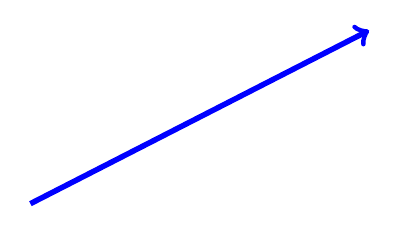
\begin{tikzpicture}[->]
\draw[draw=blue,solid,line width=0.7mm] (0, 0) -- + (4.3, 2.2);
\end{tikzpicture}}

\put(190,160){
\begin{minipage}{0.4\linewidth}
An excess of $\gamma$, due to the thermal photons generated by the fireball, is expected
\end{minipage}}

\put(260,120){

\begin{tikzpicture}[->]
\draw[draw=blue,solid,line width=0.7mm] (0, 0) -- + (0, -0.7);
\end{tikzpicture}}

\put(190,90){
\begin{minipage}{0.4\linewidth}
the ratio between gamma conversion and Dalitz decays should be larger
\end{minipage}}

\end{picture}
\end{frame}


\begin{comment}
\begin{frame}
\frametitle{Quick look into proton-proton data} 
\begin{picture}(320,250)

\put(-20,40){\includegraphics[scale=0.35]{ppdata.pdf}}

\put(-20,235){
\begin{minipage}{0.8\linewidth}
\begin{itemize}
 \item Real proton-proton data at $\sqrt{s} = 7 TeV$
\end{itemize}
\end{minipage}}

\put(220,235){
\begin{minipage}{0.8\linewidth}
HFE output
\end{minipage}}

\put(193,237){
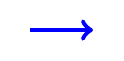
\begin{tikzpicture}[->]
\draw[draw=blue,solid,line width=0.6mm] (0, 0) -- + (0.8, 0);
\end{tikzpicture}}

\put(-10,220){
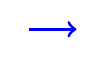
\begin{tikzpicture}[->]
\draw[draw=blue,solid,line width=0.4mm] (0, 0) -- + (0.6, 0);
\end{tikzpicture}}

\put(-10,205){
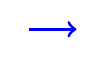
\begin{tikzpicture}[->]
\draw[draw=blue,solid,line width=0.4mm] (0, 0) -- + (0.6, 0);
\end{tikzpicture}}

\put(-10,190){
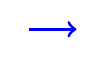
\begin{tikzpicture}[->]
\draw[draw=blue,solid,line width=0.4mm] (0, 0) -- + (0.6, 0);
\end{tikzpicture}}

\put(15,218){
\begin{minipage}{0.8\linewidth}
\footnotesize
different cuts
\end{minipage}}

\put(15,203){
\begin{minipage}{0.8\linewidth}
\footnotesize
different range and binning
\end{minipage}}

\put(15,188){
\begin{minipage}{0.8\linewidth}
\footnotesize
efficiency taken into account
\end{minipage}}

\put(90,140){
\begin{minipage}{1\linewidth}
\begin{table}[htpb]
\center
\scalebox{0.45}{
\begin{tabular}{|c|c|c|}
  \hline
  \raisebox{0pt}[15pt][12pt]{} &
  \raisebox{0pt}[15pt][12pt]{MC truth} &
  \raisebox{0pt}[15pt][12pt]{real data} \\
  \hline
  \raisebox{0pt}[15pt][12pt]{$M_{\gamma}$} &
  \raisebox{0pt}[15pt][12pt]{0.01107 $\pm$ 0.00018 $GeV/c^{2}$} &
  \raisebox{0pt}[15pt][12pt]{0.0001 $GeV/c^{2}$ - fixed} \\
  \hline
  \raisebox{0pt}[15pt][12pt]{$M_{\pi^{0}}$} &
  \raisebox{0pt}[15pt][12pt]{0.1611 $\pm$ 0.0003 $GeV/c^{2}$} &
  \raisebox{0pt}[15pt][12pt]{0.13957 $GeV/c^{2}$ - fixed} \\
  \hline
  \raisebox{0pt}[15pt][12pt]{$M_{\eta}$} &
  \raisebox{0pt}[15pt][12pt]{0.558 $\pm$ 0.004 $GeV/c^{2}$} &
  \raisebox{0pt}[15pt][12pt]{0.54785 $GeV/c^{2}$ - fixed} \\
  \hline
  \raisebox{0pt}[15pt][12pt]{$I_{\gamma}/I_{\pi^{0}}$} &
  \raisebox{0pt}[15pt][12pt]{1.19 $\pm$ 0.02} &
  \raisebox{0pt}[15pt][12pt]{1.41 $\pm$ 0.08} \\
  \hline
  \raisebox{0pt}[15pt][12pt]{$I_{\gamma}/I_{\eta}$} &
  \raisebox{0pt}[15pt][12pt]{10.0 $\pm$ 0.8} &
  \raisebox{0pt}[15pt][12pt]{6 $\pm$ 1} \\
  \hline
  \raisebox{0pt}[15pt][12pt]{$I_{\gamma}/(I_{\pi^{0}}+I_{\eta})$} &
  \raisebox{0pt}[15pt][12pt]{1.07 $\pm$ 0.02} &
  \raisebox{0pt}[15pt][12pt]{1.14 $\pm$ 0.07} \\  
  \hline
  \end{tabular}}
\end{table}
\end{minipage}}

\end{picture}
\end{frame}
\end{comment}



\end{document}